\begin{table*}[t]
\caption{Primary comparison, HE $-$ S*. Primary columns: means of 25 fold-level differences with 95\% CI; $p$ is Holm-adjusted within each protocol. Robustness columns (secondary or post hoc): conditional removal (25 folds), held-out repetitions 2--5 (20 folds), KernelSHAP and tuned components (repetition 1, 5 folds). $^*p<0.05$, unadjusted}
\label{tab:main}
\centering\footnotesize
\begin{tabular}{@{}lrrrrrrr@{}}
\toprule
 & \multicolumn{3}{c}{Primary (confirmatory)} & \multicolumn{4}{c}{$\Delta$NDF, robustness} \\
\cmidrule(lr){2-4}\cmidrule(lr){5-8}
Dataset & $\Delta$AUC & $\Delta$NDF [95\% CI] & $p$ (Holm) & Conditional & Held-out reps & KernelSHAP & Tuned \\
\midrule
\input{tab_main.tex}
\bottomrule
\end{tabular}\\[2pt]
{\scriptsize $^\dagger$CDC: separate single-dataset protocol, unadjusted. DL: DerSimonian--Laird. HKSJ: Hartung--Knapp--Sidik--Jonkman (computed for the confirmatory outcomes only). Holm-adjusted values are capped at 1.}
\end{table*}

\begin{figure*}[t]
\centering
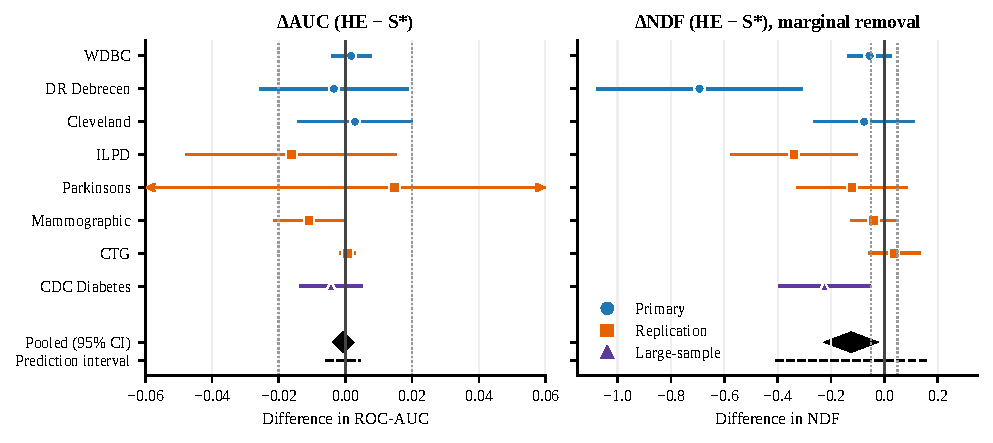
\includegraphics[width=\textwidth]{fig_forest.pdf}
\caption{Per-dataset and pooled differences (HE $-$ S*) with 95\% CI. Left: AUC. Right: NDF under marginal removal. Marker shape and color give the protocol; the diamond is the random-effects pooled estimate and the dashed line the 95\% prediction interval; arrows mark intervals that extend beyond the axis. Dotted lines: pre-specified margins of practical interest ($\pm0.02$ AUC, $\pm0.05$ NDF).}
\label{fig:forest}
\end{figure*}

\section{Results}
\subsection{Discrimination and faithfulness (confirmatory)}
HE did not improve discrimination on any dataset; the pooled AUC difference was \Nauc{} (95\% CI \NaucciL{} to \NaucciH{}; Table~\ref{tab:main}, Fig.~\ref{fig:forest}). Under marginal removal its explanations were less faithful on seven of eight datasets, significantly on diabetic retinopathy (\NpDR, Holm $p\NpDRholm$), liver disease (\NpILPD, Holm $p\NpILPDholm$) and the CDC sample (\NpCDC, $p\NpCDCholm$); no dataset favored HE significantly. The DerSimonian--Laird pooled difference was \Nndf{} (95\% CI \Nndfci; $p\Nndfp$; $I^2=\NndfI\%$), beyond the 0.05 margin of practical interest. Because this method is anti-conservative with few studies, we also computed the HKSJ interval, \Nndfhk{} ($p\Nndfhkp$), and the 95\% prediction interval, \Nndfpi{} (post hoc). The deficit is thus consistent in direction but variable in size, and pooled significance depends on the meta-analysis method.

In the primary analysis the median NDF of included patients was \Nmedhe{} for HE and \Nmeds{} for S*, and HE had the lower NDF for \Nsharelower\% of patients (\NshareDR\% on diabetic retinopathy). In the component analysis (repetition 1), deleting the top-ranked feature removed on average \NtoponeHE\% of HE's prediction gap and \NtoponeS\% of S*'s, versus about \NrandoneS\% for one random feature; deleting the top $K$ removed \NtopKHE\% and \NtopKS\% versus \NrandKS\% for $K$ random features. Shares above 100\% are common (\NoverLR\% of patients for LR): deleting a few top features marginally pushes the prediction past its all-features-deleted value, direct evidence of the off-distribution extrapolation that marginal removal induces \cite{hooker_mentch}. Of \Nnsamp{} sampled patients, \Nexclhe{} (HE) and \Nexcls{} (S*) had $G<0.05$, leaving \Nninc; exclusions were heavy for liver disease and the CDC sample (Supplement S2). With gap thresholds of 0.02 and 0.10 (post hoc), the same three datasets remained significant and the pooled difference was \Nthrtwo{} (HKSJ \Nthrtwohk) and \Nthrten{} (HKSJ \Nthrtenhk). HE's gaps were slightly smaller (median \NGhe{} vs \NGs), but patients with similar gaps showed a similar deficit (\NsimG).

\subsection{Ensembling or non-additive models? (secondary and post hoc)}
The marginal-removal deficit was robust to held-out repetitions (\Nheldout, $p\Nheldoutp$), to KernelSHAP (\Nkernel{} vs \Nperm{} with permutation SHAP on repetition 1) and to tuning (\Ntunndf, $p\Ntunndfp$; Table~\ref{tab:main}). After tuning, S* was SVM, RF or XGB in \Nnlfoldsall{} of \Ntunfolds{} folds (\Nnlfoldsused{} with included patients). With a dataset random intercept, HE's deficit in those folds was \Nnlmix{} (95\% CI \Nnlmixci; $p\Nnlmixp$), smaller and borderline compared with folds where S* was LR (\Nlmix; Table~\ref{tab:robust}). The component analysis is clearer. Median NDF on repetition 1 was \NmedLR{} (LR), \NmedXGB{} (XGB), \NmedSVM{} (SVM), \NmedKNN{} (KNN), \NmedRF{} (RF) and \NmedHE{} (HE); HE was less faithful than XGB (\NHExgb, $p\NHExgbp$) but not than RF (\NHErf), and XGB was as faithful as LR (\NXGBlr). The deficit is therefore not simply ``tree versus linear''. The standard stacking ensemble showed a smaller deficit against S* (\NSTs, $p\NSTsp$) and soft voting a non-significant one (\NSVs). TreeSHAP agreed with permutation SHAP (rank correlation $\ge$\Ntreerho) and Monte-Carlo error was small (Supplement S4--S6). Faithfulness correlation (FC) \cite{bhatt} was lower for HE on average (\Nbhatt, $p\Nbhattp$) but heterogeneous ($I^2=\NbhattI\%$) and, notably, \emph{higher} for HE on diabetic retinopathy (\NFCDR, $p\NFCDRp$), where NDF showed the largest deficit. FC rewards a linear relation between summed attribution and output change over random subsets, which spreading credit over near-duplicate counts can raise, whereas NDF rewards removing the prediction quickly with the top-ranked features; the two metrics therefore capture different properties (Supplement S7).

\begin{table}[t]
\caption{Robustness of the deficit (secondary and post hoc): pooled $\Delta$NDF over eight datasets, repetition 1}
\label{tab:robust}
\centering\scriptsize
\resizebox{\columnwidth}{!}{\begin{tabular}{@{}lrrrr@{}}
\toprule
 & \multicolumn{2}{c}{Marginal removal} & \multicolumn{2}{c}{Conditional} \\
\cmidrule(lr){2-3}\cmidrule(lr){4-5}
Comparison & $\Delta$NDF [95\% CI] & $p$ & $\Delta$NDF & $p$ \\
\midrule
\input{tab_robust.tex}
\bottomrule
\end{tabular}}\\[2pt]
{\scriptsize SV, ST: soft-voting and stacking ensembles of all five components. Comparison rows: DerSimonian--Laird. Tuned rows: fold means with a dataset random intercept.}
\end{table}

\subsection{Removal operator and simulation (secondary)}
For untuned models, the pooled difference under conditional removal was smaller, \Nknn{} ($p\Nknnp$); on diabetic retinopathy it shrank from \NpDR{} to \NpDRknn. With tuned components, however, a substantial conditional deficit remained (fold means with a dataset random intercept: \Ntunallmixk, $p\Ntunallmixkp$, versus \Ntunallmix{} marginal; \Nnlmixk{} when S* was non-linear), and HE was less faithful than RF only under conditional removal (Table~\ref{tab:robust}). The operator therefore modulates the deficit for untuned models but does not explain it in general; we did not investigate why tuning changes this. In the simulation (Supplement S9), the marginal-removal deficit of HE relative to LR grew with within-block correlation under a linear outcome (\NsimLzero, \NsimLhalf{} and \NsimLnine{} at $\rho=0$, 0.5, 0.9) but stayed near zero under conditional removal (interaction \Nsimint, SE \Nsimintse; $p\Nsimintp$).

\subsection{Correlation-aware remedy}
In the exploratory discovery analysis, attributing to clusters of correlated features narrowed the deficit. The pre-specified test on held-out repetitions (Table~\ref{tab:remedy}) confirmed this where large correlated blocks exist: on diabetic retinopathy the deficit fell from \NdfeatDR{} to \NdgrpDR{} (reduction \NRDR, $p\NRDRp$), and correlation clusters outperformed random clusters of the same sizes (\NPLDR, $p\NPLDRp$); reductions were also significant on liver disease (\NRILPD) and WDBC (\NRWDBC). The pre-specified pooled hypothesis was not supported (pooled reduction \NpoolR, $p\NpoolRp$): clustering enlarged the gap on cardiotocography (\NRCTG), and over all datasets correlation clusters did no better than random ones (\NpoolPL, $p\NpoolPLp$). A pre-specified non-additivity explanation for the remaining deficit was also not supported (Supplement S8).

\begin{table}[t]
\caption{Remedy: $\Delta$NDF (HE $-$ S*) with feature- and cluster-level attribution. Discovery: repetition 1. Confirmation: held-out repetitions 2--5}
\label{tab:remedy}
\centering\scriptsize
\setlength{\tabcolsep}{2.5pt}
\begin{tabular}{@{}lrrrrr@{}}
\toprule
 & Discovery & \multicolumn{4}{c}{Confirmation (pre-specified)} \\
\cmidrule(lr){2-2}\cmidrule(lr){3-6}
Dataset & Reduction & $\Delta$NDF feature & $\Delta$NDF cluster & Reduction $R$ & Placebo \\
\midrule
\input{tab_remedy.tex}
\bottomrule
\end{tabular}\\[2pt]
{\scriptsize Reduction = cluster $-$ feature $\Delta$NDF; Placebo = reduction with correlation clusters minus reduction with random clusters of the same sizes. $^*p<0.05$.}
\end{table}
